% !TeX document-id = {87432cc9-c386-48dc-9558-b3c42a74a150}
% !TEX encoding = UTF-8
% !TEX TS-program = pdflatex
% !TEX spellcheck = it-IT
%% !TEX root = 
% !BIB TS-program = biber
% Comandi speciali (o righe magiche) trattati come commenti da Latex ma non da 
%editor come Texstudio e Texshop, che si impostano di conseguenza. In ordine:
% dichiara la codifica dei caratteri con cui impostare l'editor (bisogna 
%comunque caricare inputenc con la stessa codifica)
% dichiara il motore di composizione (pdflatex o lualatex)
% attiva il controllo ortografico della lingua del documento
% dichiara la condizione di file principale e di file secondario nei documenti 
%suddivisi in più file
% imposta biber come motore bibliografico

\documentclass[9pt]{extarticle}


% ------------------------------------------------------------------------------
% Packages
% ------------------------------------------------------------------------------
\usepackage[utf8]{inputenc}
\usepackage{graphicx}
\usepackage{amsmath}
\usepackage{amssymb}
\usepackage{amsthm}
\usepackage{hyperref}
\usepackage{titlesec}
\usepackage{parskip}
\usepackage{float}
\usepackage{booktabs}
\usepackage{caption}
\usepackage{blindtext}
\usepackage[table,xcdraw]{xcolor}
\usepackage{enumitem}
% Define a new counter for functional requirements
\newcounter{rf}
\newcommand{\FR}{\refstepcounter{rf}\textbf{FR\therf: }}
% Define a new counter for non-functional requirements
\newcounter{nonfunc}
\newcommand{\NONFUNC}{\refstepcounter{nonfunc}\textbf{NFR\thenonfunc: }}

% ------------------------------------------------------------------------------
% Page setup
% ------------------------------------------------------------------------------
\usepackage{geometry} 
\geometry{a4paper, margin=1in, twoside}
\usepackage{setspace}
\setstretch{1.2}  % Adjust the number as needed
%\doublespacing


% ------------------------------------------------------------------------------
% Referencing
% ------------------------------------------------------------------------------
\usepackage[
	backend=biber,
	citestyle=authoryear,
	bibstyle=authoryear,
	maxcitenames=2,
	maxbibnames=99]{biblatex}
%\addbibresource{references.bib}
%\DeclareNameAlias{sortname}{family-given}
%\setlength\bibitemsep{1em}

% ------------------------------------------------------------------------------
% Code listings
% ------------------------------------------------------------------------------
\usepackage{listings}
\usepackage{xcolor}
\lstdefinestyle{matlabcode}{
	backgroundcolor=\color{gray!10},   
	commentstyle=\color{green!50!black},
	keywordstyle=\color{blue},
	stringstyle=\color{magenta},
	basicstyle=\linespread{1}\footnotesize\ttfamily,
	numberstyle=\tiny,
	breakatwhitespace=false,         
	breaklines=true,                 
	captionpos=t,   
	frame=single,
	keepspaces=true,         
	language=matlab,        
	numbers=none,             
	numbersep=5pt,                  
	showspaces=false,                
	showstringspaces=false,
	showtabs=false,                  
	tabsize=2,
	aboveskip=1em,
	belowskip=1em,
	belowcaptionskip=12pt
}

% ------------------------------------------------------------------------------
% Headers and footers
% ------------------------------------------------------------------------------	
\usepackage{fancyhdr}
\pagestyle{fancy}   
\setlength{\headheight}{14.5pt}
\renewcommand{\headrulewidth}{0.3pt}
%\renewcommand{\chaptermark}[1]{\markboth{\chaptername\ \thechapter.\ #1}{}}
\renewcommand{\sectionmark}[1]{\markright{\thesection.\ #1}}   
\fancyhead[LE,RO]{\rightmark}
\fancyhead[LO,RE]{\leftmark}

% ------------------------------------------------------------------------------
% Title page
% ------------------------------------------------------------------------------

\newcommand{\name}{Togni Roberto}
\newcommand{\projecttitle}{EvenTrento}
\newcommand{\course}{Ingegneria del Software}
\newcommand{\customtitle}{
	\vspace*{1cm}
	\begin{center}
		
\includegraphics[width = 7cm]{images/logo_rosso} \\
		\vspace{1cm}
	\end{center}
	\LARGE{Progetto:}
	\begin{center}
%		\vspace{2cm}
		\textbf{\Huge{\projecttitle}} \\
	\end{center}
	\LARGE{Titolo del documento:}
	\begin{center}
%		\vspace{1cm}
		\textbf{\Huge Descrizione di Progetto} \\
	\end{center}
	\LARGE{Autore:}
	\begin{center}
		%		\vspace{1cm}
		\textbf{\name} \\
	\end{center}
	\vspace{1cm}
	Document Info:
	
	\begingroup
	\setlength{\tabcolsep}{10pt} % Default value: 6pt
	\renewcommand{\arraystretch}{1.5}
	
	\begin{table}[!htb]
		\begin{tabular}{lllll}
			\cline{1-4}
			\cellcolor[HTML]{13315C}{\color[HTML]{FFFFFF} Doc. Name}                         & D1-EvenTrentoDescrizioneProgetto & \multicolumn{1}{l|}{\cellcolor[HTML]{13315C}{\color[HTML]{FFFFFF} Doc. Number}} & \multicolumn{1}{l|}{D1 V0.1} &  \\ \cline{1-4}
			\multicolumn{1}{|l|}{\cellcolor[HTML]{13315C}{\color[HTML]{FFFFFF} Description}} & \multicolumn{3}{l|}{Documento di analisi dei requisiti funzionali, non funzionali e front-end}                                                    &  \\ \cline{1-4}
			&                                  &                                                                                 &                              &  \\
			&                                  &                                                                                 &                              &  \\
		\end{tabular}
	\end{table}
	
	\endgroup
	
	\begin{center}
		\vfill 
		\textbf{\Large Dipartimento di Ingegneria e Scienza dell'Informazione}
		\vspace{1cm}
	\end{center}
	\newpage
	\pagenumbering{roman}
	\setcounter{page}{0}
}

% ------------------------------------------------------------------------------
% Theorem enivornments
% ------------------------------------------------------------------------------
%\newtheorem{theorem}{Theorem}[chapter]
%\newtheorem{definition}{Definition}[chapter]
%\newtheorem{corollary}{Corollary}[theorem]
%\newtheorem{lemma}[theorem]{Lemma}

\newtheoremstyle{break}%
    {}{}%
    {}{}%
    {\bfseries}{}% % Note that final punctuation is omitted.
    {\newline}{}
\theoremstyle{break}
%\newtheorem{example}{Example}[chapter]



% ------------------------------------------------------------------------------
% Document
% ------------------------------------------------------------------------------


\begin{document}
\customtitle



% TODO add chapters
\tableofcontents
\newpage

\section{Scopo del Documento}

Il presente documento ha lo scopo di riportare le informazioni riguardanti lo
sviluppo di una parte dell'applicazione EvenTrento. Partendo dalle user stories,
il documento presenta un walk-throgh delle funzionalità effettivemente
implementate, con un focus sull'interazione dell'utente con queste ultime.
Prosegue dunque con la descrizione delle web APIs del'applicazione, nonché
della modalità di sviluppo collaborativo, del database e del testing delle varie
funzionalità.
Infine, viene presentato il front-end realizzato, accompagnato da una
descrizione della modalità di deployment utilizzata.

\newpage

\section{User Stories}

Le seguenti tabelle raccolgono una sere di User Stories divise in diverse epiche. Ad ogni user story è associata una priorità (ad un numero più piccolo corrisponde una priorità maggiore) rappresentante l'importanza della funzionalità in questione per l'operatività del sistema.

	
\begin{table}[!htb]
	\centering
	\begin{tabular}{clp{7cm}l} % Use 'p{7cm}' for the User Story column
		\toprule
		\multicolumn{4}{c}{\textbf{Profilo}}\\ \midrule
		Id & Nome & User Story & Priorità \\ \midrule
		A1  & Registrazione  & Come utente, voglio registrarmi per utilizzare il sistema & 1 \\
		A2  & Login & In qualità di utente, devo essere in grado di effettuare il login & 1 \\
		A3  & Visualizzazione profilo & Come utente, devo essere in grado di visualizzare lo storico eventi, le mie informazioni personali, e gli eventi salvati &  2\\
		\bottomrule
	\end{tabular}
	\caption{User stories relative all'epica "profilo".}
	\label{tab:profili}
\end{table}


\begin{table}[!htb]
	\centering
	\begin{tabular}{clp{7cm}l} % Use 'p{7cm}' for the User Story column
		\toprule
		\multicolumn{4}{c}{\textbf{Eventi}}\\ \midrule
		Id & Nome & User Story & Priorità \\ \midrule
		B1  & Lista eventi            & In qualità di utente, devo essere in grado di scorrere una lista di eventi                                               &  2\\
		B2  & Filtri eventi           & In qualità di utente, devo essere in grado di filtrare gli eventi in base alla data                                      &  2 \\
		B3  & Creazione evento        & In qualità di organizzatore, devo essere in grado di creare un nuovo evento in un determinato luogo                      &  2 \\
		B4  & Condivisione evento     & In qualità di utente, devo essere in grado di condividere un evento tramite link                                         &  4\\
		B5  & Pagamento               & In qualità di utente, devo essere in grado di effettuare il pagamento per un evento a cui voglio iscrivermi              & 2\\
		B6  & Aggiornamento evento    & In qualità di organizzatore, devo essere in grado di aggiornare la descrizione di un evento                              & 3\\
		B7  & Statistiche evento      & In qualità di organizzatore, devo essere in grado di visualizzare gli iscritti all'evento                                & 4\\
		B8  & Salvataggio evento      & In qualità di utente, devo essere in grado di salvare un evento in modo da poterlo visualizzare nella mia area personale & 3\\
		\bottomrule
	\end{tabular}
	\caption{User stories relative all'epica "eventi".}
	\label{tab:eventi}
\end{table}

\begin{table}[!htb]
	\centering
	\begin{tabular}{clp{7cm}l} % Use 'p{7cm}' for the User Story column
		\toprule
		\multicolumn{4}{c}{\textbf{Spazi}}\\ \midrule
		Id & Nome & User Story & Priorità \\ \midrule
		C1  & Aggiunta spazio  & In qualità di owner, devo essere in grado di pubblicare uno spazio disponibile & 2\\
		C2 & Rimozione spazio & In qualità di owner, devo essere in grado di rimuovere uno spazio esistente & 2\\
		C3 & Visualizzazione spazi & In qualità di organizzatore, devo essere in grado di visualizzare gli spazi disponibili & 3\\
		\bottomrule
	\end{tabular}
	\caption{User stories relative all'epica "spazi".}
	\label{tab:spazi}
\end{table}



\begin{table}[!htb]
	\centering
	\begin{tabular}{clp{7cm}l} % Use 'p{7cm}' for the User Story column
		\toprule
		\multicolumn{4}{c}{\textbf{Mappa}}\\ \midrule
		Id & Nome & User Story & Priorità \\ \midrule
		D1  & Esplorazione mappa      & In qualità di utente, devo essere in grado di muovermi nella mappa per visualizzare gli eventi                           & 1 \\
%		D2  & Aggiunta luogo          & In qualità di owner, devo essere in grado di aggiungere un nuovo luogo alla mappa                                        & \\
		\bottomrule
	\end{tabular}
	\caption{User stories relative all'epica "mappa".}
	\label{tab:mappa}
\end{table}

\newpage
\section{User Flow}

Di seguito sono riportati i diagrammi di flusso rappresentanti gli user flow corrispondenti ad una serie di user stories. La notazione utilizzata nelle descrizioni si riferisce a quella riportata nelle Tabelle \ref{tab:profili}, \ref{tab:eventi}, \ref{tab:spazi} e \ref{tab:mappa}.

\begin{figure}[!htb]
	\centering
	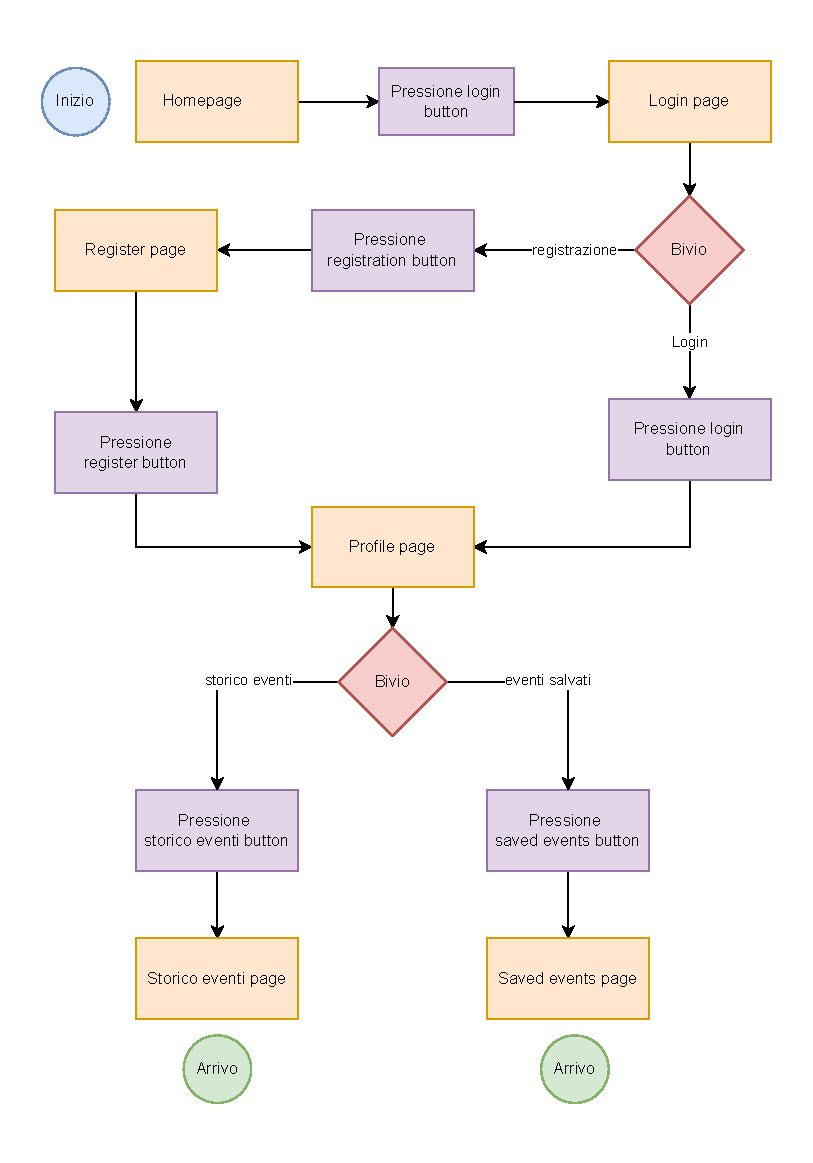
\includegraphics[width=0.7\linewidth]{./images/A1-A2-A3.pdf}
	\caption{User Flowchart relativo alle user stories A1, A2 e A3.}
	\label{fig:A1-A2}
\end{figure}

\newpage 

\begin{figure}[!htb]
	\centering
	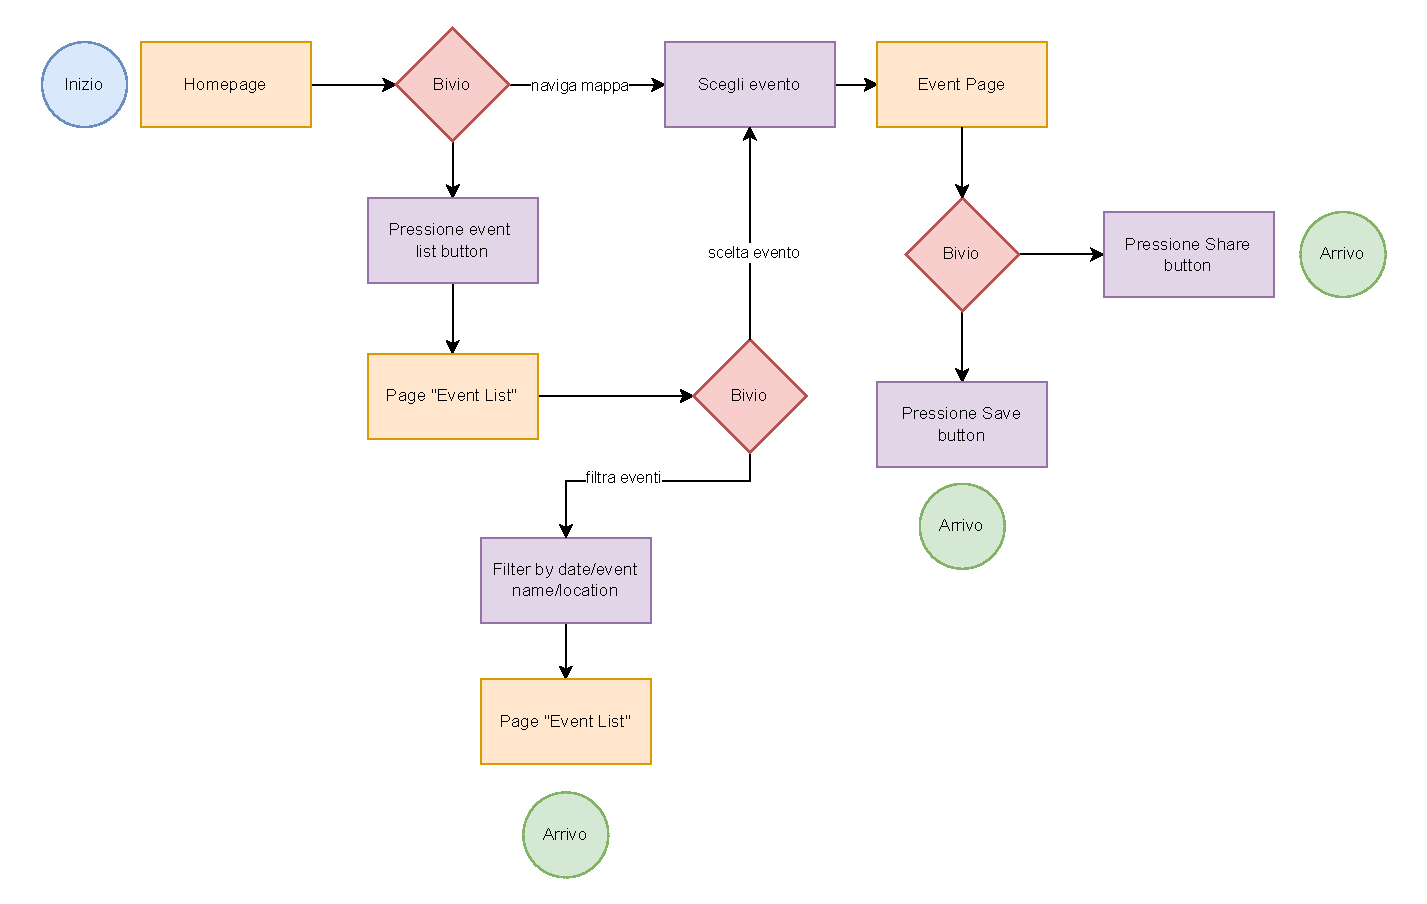
\includegraphics[width=\linewidth]{./images/B1-B2-B4-B8-D1.pdf}
	\caption{User Flowchart relativo alle user stories B1, B2, B4, B8 e D1.}
	\label{fig:B1-C1}
\end{figure}


\begin{figure}[!htb]
	\centering
	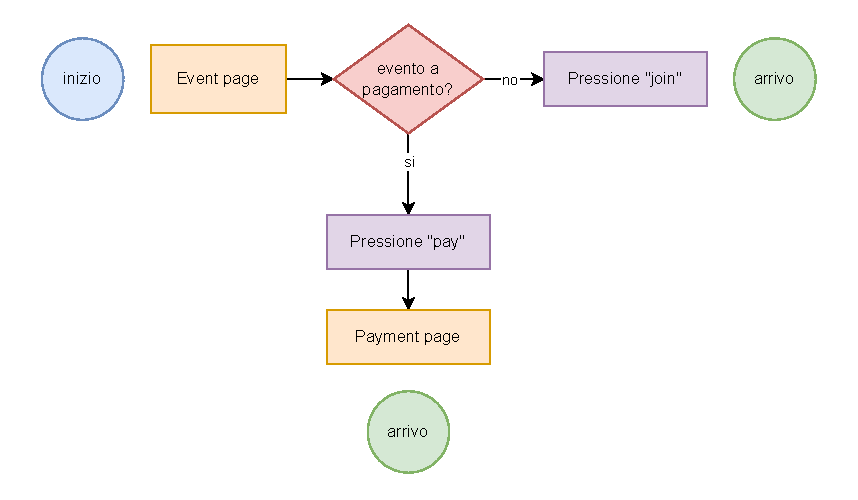
\includegraphics[width=0.8\linewidth]{./images/B5.pdf}
	\caption{User Flowchart relativo alla user story B5.}
	\label{fig:B5}
\end{figure}

\newpage  

\begin{figure}[!htb]
	\centering
	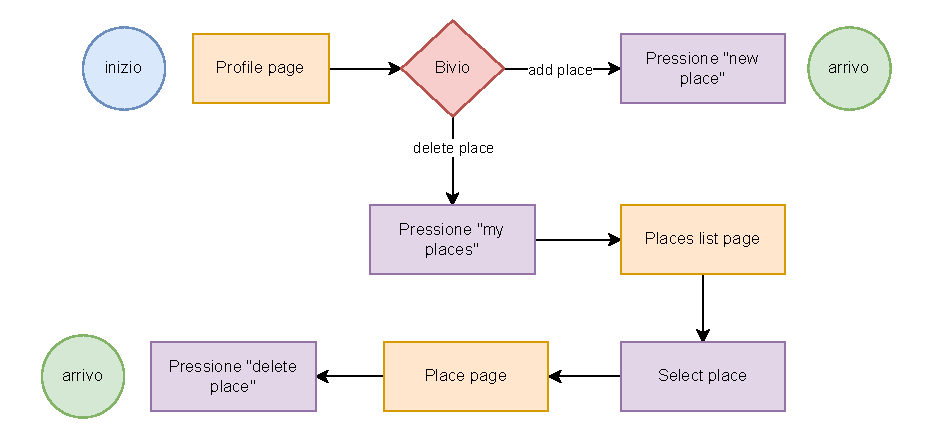
\includegraphics[width=0.8\linewidth]{./images/C1-C2.pdf}
	\caption{User Flowchart relativo alle user stories C1 e C2.}
	\label{fig:C1-C2}
\end{figure}

\begin{figure}[!htb]
	\centering
	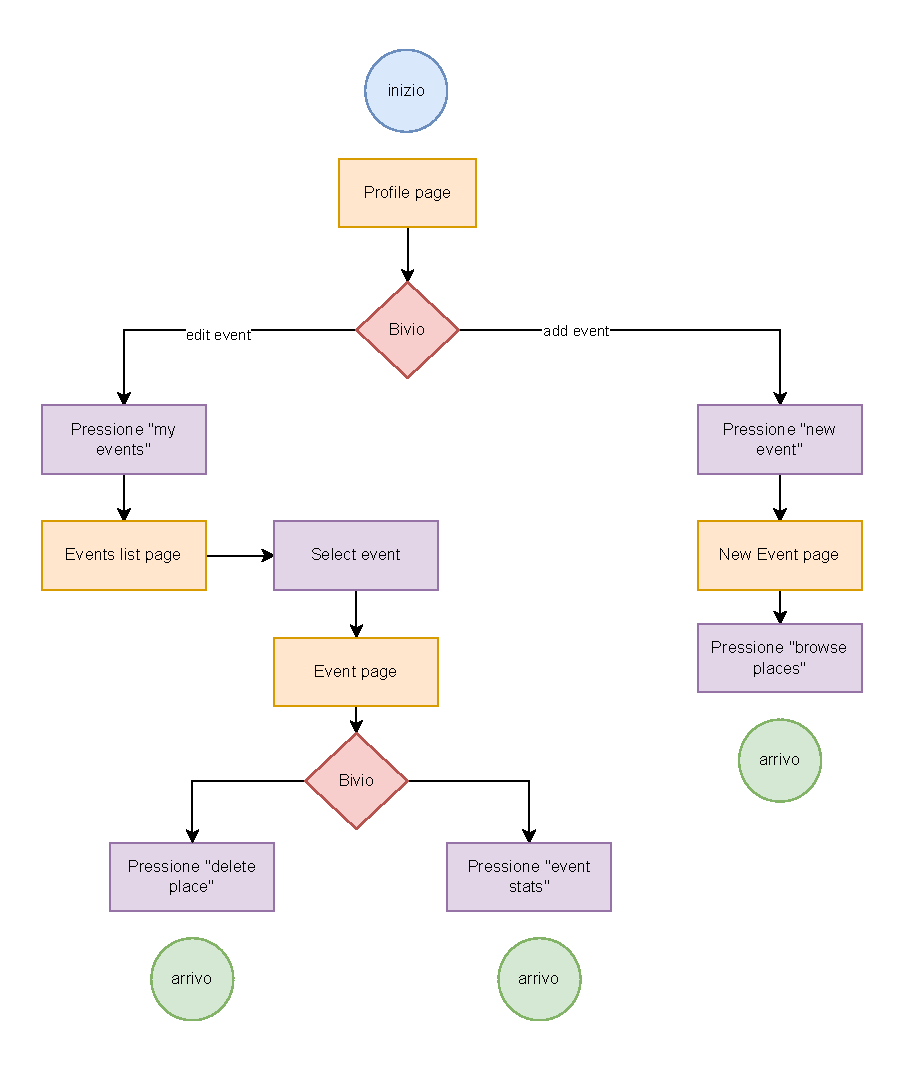
\includegraphics[width=0.8\linewidth]{./images/B3-B6-B7-C3.pdf}
	\caption{User Flowchart relativo alle user stories B3, B6, B7 e C3.}
	\label{fig:B3-B6-B7-C3}
\end{figure}

\newpage
\section{Web APIs}

Le API sono state documentate rispettando le specifiche openapi3. La specifica è disponibile nella \href{https://github.com/rtogni00/IS\_Progetto}{repository GitHub}, ed è per comodità riportata di seguito.

\begin{lstlisting}[style=yamlcode, caption={Documentazione API}]
	openapi: 3.0.0
	info:
		version: 1.0.0
		title: "EvenTrento OpenAPI 3.0"
		description: API for managing events.
		license:
		name: MIT
	servers:

		- description: Localhost
		url: http://localhost:8000/api/v1
	
	##################
	# API ENDPOINTS
	##################
	
	paths:
	# path per gestire la registrazione di un utente
	/users/signup:
		post:
			description: >-
				Creates a new user in the system.
			summary: Register a new user
			requestBody:
			required: true
				content:
					application/json:
						schema:
							$ref: '#/components/schemas/User'
			responses:
				"201":
					description: "User created. Link in the Location header"
					headers:
						"Location":
							schema:
								type: string
								description: Link to the newly created student.
				"400":
					description: "Invalid input. Please verify the request body."
				"409":
					description: "User already exists."
				
	# path per gestire il login di un utente gia' registrato
	/users/login:
		post:
			summary: Login to the system
			description: Authenticate the user and return a JWT token.
			requestBody:
				required: true
				content:
					application/json:
						schema:
							type: object
							properties:
								email:
									type: string
									description: "Email address of the user"
								password:
									type: string
									description: "Password for the user account"
							required:
								- email
								- password
			responses:
				'200':
					description: Login successful
					content:
						application/json:
							schema:
								type: object
								properties:
									token:
										type: string
										description: "JWT token to authenticate future requests"
				'400':
					description: Invalid email or password
				'500':
					description: Internal server error
	
	# path per gestire gli eventi salvati dall'utente
	/users/saved-events:
		post:
			summary: Save an event of interest for a user
			description: Allows a user to save an event they are interested in.
			security:
				- bearerAuth: []   # Richiede un token JWT valido per accedere
			requestBody:
				required: true
				content:
					application/json:
						schema:
							type: object
							properties:
								eventId:
									type: integer
									description: The ID of the event to save
								userId:
									type: integer
									description: The ID of the user saving the event
			responses:
				'201':
					description: 'Event saved successfully'
					content:
						application/json:
							schema:
								type: object
								properties:
									message:
										type: string
			'404':
				description: 'Event not found'
			'400':
				description: 'Invalid save request'
			'500':
				description: 'Internal server error'
		get:
			summary: Retrieve saved events for the authenticated user
			description: Returns a list of events saved by the authenticated user.
			security:
				- bearerAuth: []
			responses:
				'200':
					description: 'List of saved events'
					content:
						application/json:
							schema:
								type: array
								items:
									$ref: '#/components/schemas/Event'
			'401':
				description: 'Unauthorized user'
			'500':
				description: 'Internal server error'
				
	# path per creare e fare il retrieving di eventi
	/events:
		get:
			description: Returns a list of events, optionally filtered by date.
			summary: View all events (with optional date filter)
			parameters:
				- in: query
					name: startDate
					schema:
						type: string
						format: date-time
					required: false
			responses:
				'200':
					description: 'Collection of events'
					content:
						application/json:
						schema:
							type: array
							items:
							$ref: '#/components/schemas/Event'
			'400':
				description: 'Invalid date format'
			'500':
				description: 'Internal server error'


	post:
		description: >-
			Creates a new event in the system.
		summary: Create a new event
		security:
			- bearerAuth: []   # Richiede un token JWT valido per accedere
		requestBody:
			required: true
			content:
				application/json:
					schema:
						$ref: '#/components/schemas/EventCreation' # Creating a new event
		responses:
			'201':
				description: 'Event successfully created'
				content:
					application/json:
						schema:
							$ref: '#/components/schemas/Event'  # Returning the created event
		'400':
			description: 'Invalid input, check the event details'
		'403':
			description: 'User not authorized to create an event (only organizers)'
		'500':
			description: 'Internal server error'
					
	# path per la modifica di un evento esistente
	/events/{eventId}:
		put:
			summary: Update an existing event
			description: Allows an organizer to update an event they created.
			security:
				- bearerAuth: []   # Richiede un token JWT valido per accedere
			parameters:
				- in: path
					name: eventId
					schema:
						type: integer
					required: true
					description: The ID of the event to be updated
			requestBody:
				required: true
				content:
					application/json:
						schema:
							$ref: '#/components/schemas/EventUpdate'  # Schema per aggiornamento
			responses:
				'200':
					description: 'Event updated successfully'
					content:
						application/json:
							schema:
								$ref: '#/components/schemas/Event'
			'403':
				description: 'Forbidden. Organizer is not authorized to modify this event.'
			'404':
				description: 'Event not found'
			'500':
				description: 'Internal server error'
				
	# path per l'iscrizione ad un evento                
	/events/{eventId}/registration:
		post:
			summary: Register a participant for an event
			description: Allows a participant to register for a specific event.
			security:
				- bearerAuth: []   # Richiede un token JWT valido per accedere
			parameters:
				- in: path
					name: eventId
					required: true
					schema:
						type: integer
			responses:
				'201':
					description: 'Registration successful'
					content:
						application/json:
							schema:
								type: object
								properties:
									message:
										type: string
			'404':
				description: 'Event not found'
			'400':
				description: 'Invalid registration request'
			'500':
				description: 'Internal server error'
			
	# path per gli spazi
	/places:
		get:
			summary: Retrieve a list of spaces
			description: Returns a list of all available spaces.
			security:
				- bearerAuth: []   # Richiede un token JWT valido per accedere
			responses:
				'200':
					description: 'A list of spaces'
					content:
						application/json:
							schema:
								type: array
								items:
									$ref: '#/components/schemas/Place'
				'500':
					description: 'Internal server error'
					
		post:
			summary: Create a new space
			description: Allows an owner to create a new space for events.
			security:
				- bearerAuth: []   # Richiede un token JWT valido per accedere
			requestBody:
				required: true
				content:
					application/json:
					schema:
						$ref: '#/components/schemas/Place'
			responses:
				'201':
					description: 'Place created successfully'
					content:
						application/json:
							schema:
								$ref: '#/components/schemas/Place'
			'400':
				description: 'Invalid input'
			'500':
				description: 'Internal server error'
				
		put:
			summary: Update an existing space
			description: Allows an owner to update a space they created.
			security:
				- bearerAuth: []   # Richiede un token JWT valido per accedere
			parameters:
				- in: path
					name: spaceId
					required: true
					schema:
						type: integer
			requestBody:
				required: true
				content:
					application/json:
						schema:
							$ref: '#/components/schemas/PlaceUpdate'
			responses:
				'200':
				description: 'Place updated successfully'
				content:
					application/json:
						schema:
							$ref: '#/components/schemas/Place'
			'403':
				description: 'Forbidden. Owner is not authorized to modify this space.'
			'404':
				description: 'Place not found'
			'400':
				description: 'Invalid input'
			'500':
				description: 'Internal server error'
				
	
	#######################
	# COMPONENTS SECTION
	#######################
	
	components:
		schemas:
			User:
				type: object
				required:
					- username
					- email
					- password
					- role
				properties:
					username:
						type: string
						description: "Username of the user"
					email:
						type: string
						description: "Email address of the user"
					password:
						type: string
						description: "Password for the user account"
					role:
						type: string
						enum: [basicUser, owner, organizer]
						description: "Role of the user in the system"
						
			Event:
				type: object
				required:
					- id
					- name
					- date
					- location
					- organizerId
				properties:
					id:
						type: integer
						description: "Unique identifier of the event"
					name:
						type: string
						description: "Name of the event"
					description:
						type: string
						description: "Brief description of the event"
					date:
						type: string
						format: date-time
						description: "Date and time of the event"
					location:
						type: string
						description: "Location where the event will be held"
					organizerId:
						type: integer
						description: "The ID of the organizer who created the event"
			
			EventCreation:
				type: object
				required:
					- name
					- date
					- location
				properties:
					name:
						type: string
						description: "Name of the event"
					description:
						type: string
						description: "Brief description of the event"
					date:
						type: string
						format: date-time
						description: "Date and time of the event"
					location:
						type: string
						description: "Location where the event will be held"
						
			EventUpdate:
				type: object
				required:
				- name
				- description
				- date
				- location
				properties:
					name:
						type: string
						description: "Updated name of the event"
					description:
						type: string
						description: "Updated description of the event"
					date:
						type: string
						format: date-time
						description: "Updated date and time of the event"
					location:
						type: string
						description: "Updated location of the event"
						
			Place: # oggetto per la creazione e la visualizzazione dello spazio
				type: object
				properties:
					id:
						type: integer
						description: Unique identifier of the space
					name:
						type: string
						description: Name of the space
					location:
						type: string
						description: Location of the space
					capacity:
						type: integer
						description: Maximum capacity of the space

   		    PlaceUpdate: # oggetto per l'aggiornamento dello spazio
				type: object
				properties:
					name:
						type: string
						description: Updated name of the space
					location:
						type: string
						description: Updated location of the space
					capacity:
						type: integer
						description: Updated maximum capacity of the space
	
			
		# modalita' di autenticazione che le API utilizzano
		securitySchemes:
			bearerAuth:
				type: http
				scheme: bearer
				bearerFormat: JWT
				
\end{lstlisting}
	

\newpage

\section{Implementation}
\subsection{Repository Implementation}

Il codice del progetto, disponibile su \href{https://github.com/rtogni00/IS_Progetto}{GitHub}, è organizzato secondo questo schema:

\begin{lstlisting}[style=treestyle, caption=Struttura della repository]
.
+-- D1
+-- D2
+-- D3
+-- D4
+-- front_end
|   +-- index.html
|   +-- pages
|   +-- scripts
|   +-- styles
+-- node_app
|   +-- app.js
|   +-- helperFunctions // funzioni ausiliarie usate durante lo sviluppo
|   +-- .env.example // esempio di file di configurazione delle
|   |                // variabili d'ambiente
|   +-- index.js
|   +-- models // modelli dati mongoose
|   +-- package.json  // file di configurazione del progetto npm
|   +-- package-lock.json
|   +-- routes  // endpoint routes per le APIs
|   +-- tokenChecker.js // middleware per l'autenticazione
+-- README.md
|   +-- .gitignore // configurazione git repo
+-- swagger
    +-- evenTrentoAPIs.yaml // documentazione API
\end{lstlisting}


\subsection{Branching strategy e organizzazione del lavoro}

Malgrado i propositi di collaborazione iniziali, verso la fine del mese di
settembre ho preso la decisione di proseguire lo sviluppo in modo individuale.
Come facilmente osservabile dalla commit history del progetto, il contributo
degli altri due membri del gruppo è limitato al processo di brainstorming e
alla realizzazione di alcuni grafici relativi allo User Flow. Tali grafici non
sono presenti nella versione finale del presente documento a causa della loro
modifica nel corso dello sviluppo dell'applicazione. Una descrizione dettagliata
delle statistiche finali è riportata in Figura \textbf{TODO}.



\begin{verbatim}
git log --format='%aN <%aE>' | sort | uniq -c | sort -nr
\end{verbatim}



\subsection{Dependencies}

Il progetto npm fa uso dei seguenti moduli:
\begin{itemize}
    \item \textbf{Cors} per il supporto alle chiamate cross-origin
    \item \textbf{Express} come framework per il backend
    \item \textbf{Jsonwebtoken} per gestire l'autenticazione
    \item \textbf{Mongoose} per interfacciarsi con mongoDB
    \item \textbf{Axios} per interagire con l'API di \href{https://www.openstreetmap.org/#map=6/42.09/12.56}{OpenStreetMap}
\end{itemize}

Sono inoltre riportate le seguenti dipendenze di sviluppo:
\begin{itemize}
    \item \textbf{Dotenv} per la gestione delle variabili d'ambiente
    \item \textbf{TODO}
\end{itemize}

\subsection{Database}

La gestione dei dati è stata realizzata basandosi su un database non
relazionale. In particolare, si è fatto uso del servizio offerto da
\href{https://www.mongodb.com/products/platform/atlas-database}{Atlas MongoDB}.

Per la gestione dei dati necessari per il funzionamento dell'applicazione sono state definite quattro strutture dati mediante Mongoose:
\begin{itemize}
	\item Event: per gestire tutte le funzionalità legate alla creazione, modifica ed eliminazione degli eventi
	\item EventRegistration: per gestire correttamente l'iscrizione e la disiscrizione degli utenti dagli eventi
	\item Place: per gestire tutte le funzionalità legate alla creazione, modifica ed elimazione dei luoghi
	\item User: per gestire le tre tipologie di utente e le attività ad esse collegate
\end{itemize}

\newpage
\subsection{Testing}

\textbf{TODO}

\section{Front-End}

\section{Deployment}

	
\end{document}
